\subsection{Riepilogo}
	\subsubsection{Ore totali}
		\subsubsubsection{Suddivisione del lavoro}
			Distribuzione totale delle ore per ciascun ruolo comprensive delle ore di investimento e delle ore rendicontate al carico del Committente\ped{\textit{G}}.

			\rowcolors{2}{lightRowColor}{darkRowColor}
			\begin{longtable}{
				>{\centering}p{0.25\textwidth}
				>{\centering}p{0.05\textwidth}
				>{\centering}p{0.05\textwidth}
				>{\centering}p{0.05\textwidth}
				>{\centering}p{0.05\textwidth}
				>{\centering}p{0.05\textwidth}
				>{\centering}p{0.05\textwidth}
				>{\centering\arraybackslash}p{0.15\textwidth} }

				\coloredTableHead
				\textbf{\color{white}Nome} &
				\textbf{\color{white}Rp} &
				\textbf{\color{white}As} &
				\textbf{\color{white}An} &
				\textbf{\color{white}Pt} &
				\textbf{\color{white}Pr} &
				\textbf{\color{white}Vf} &
				\textbf{\color{white}Totale}
				\tabularnewline
				\endhead

				% Contenuto della tabella
				% Nome & Rp & As & An & Pt & Pr & Vf & Totale \\
				\VB & 17 & 24 & 3  & 19 & 34 & 40 & 137 \\
				\LB & 10 & 26 & 10 & 26 & 35 & 30 & 137 \\
				\NF & 5  & 28 & 6  & 37 & 26 & 35 & 137 \\
				\EG & 6  & 13 & 37 & 30 & 26 & 28 & 140 \\
				\FJ & 11 & 17 & 3  & 28 & 31 & 47 & 137 \\
				\MP & 30 & 14 & 2  & 23 & 22 & 46 & 137 \\
				\AS & 6  & 15 & 2  & 21 & 31 & 62 & 137 \\
				\AZ & 7  & 12 & 40 & 14 & 34 & 33 & 140 \\
				\textbf{Ore totali per ruolo} & 92 & 149 & 103 & 198 & 239 & 321 & 1102 \\

				\rowcolor{white}\caption {Suddivisione oraria con il totale delle ore di investimento e rendicontate}	\\

			\end{longtable}

			\newpage
			% Grafico
			Rappresentazione grafica della suddivisione oraria:
			\begin{figure}[h]
				\centering
				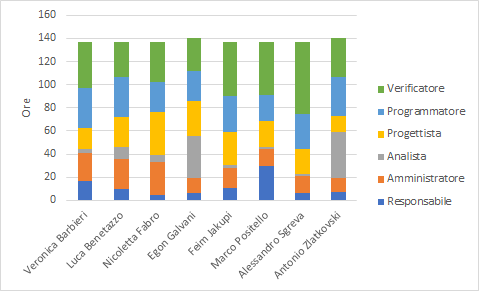
\includegraphics[width=0.7\textwidth]{./res/img/totale_po.png}
				\caption{Suddivisione oraria con il totale delle ore di investimento e rendicontate}
			\end{figure}

		\subsubsubsection{Prospetto economico}
			Totale delle ore e costo per ciascun ruolo comprensivo delle ore di investimento e delle ore rendicontate a carico del Committente\ped{\textit{G}}:

			\rowcolors{2}{lightRowColor}{darkRowColor}
			\begin{longtable}{
				>{\centering}p{0.25\textwidth}
				>{\centering}p{0.05\textwidth}
				>{\centering\arraybackslash}p{0.15\textwidth} }

				\coloredTableHead
				\textbf{\color{white}Ruolo} &
				\textbf{\color{white}Ore} &
				\textbf{\color{white}Costo in \euro{}}
				\tabularnewline
				\endhead

				% Contenuto della tabella
				% Ruolo & Ore & Costo in \\
				Responsabile    & 92   & 2.760,00 \\
				Amministratore  & 149  & 2.980,00 \\
				Analista        & 103  & 2.575,00 \\
				Progettista     & 198  & 4.356,00 \\
				Programmatore   & 239  & 3.585,00 \\
				Verificatore    & 321  & 4.815,00 \\
				\textbf{Totale} & 1102 & 21.071,00 \\

				\rowcolor{white}\caption {Prospetto dei costi totale delle ore di investimento e rendicontate per ciascun ruolo} \\

			\end{longtable}

			\newpage
			% Grafico
			Rappresentazione grafica della distribuzione dei ruoli:
			\begin{figure}[h]
				\centering
				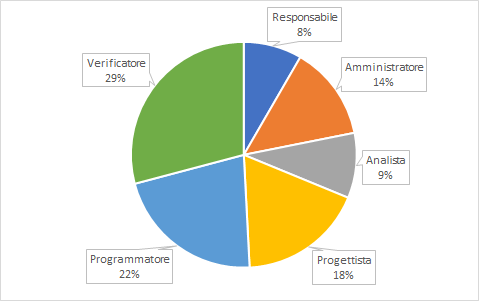
\includegraphics[width=0.7\textwidth]{./res/img/totale_pe.png}
				\caption{Suddivisione dei ruoli per il totale delle ore di investimento e rendicontate }
			\end{figure}

	\subsubsection{Ore rendicontate}
		\subsubsubsection{Suddivisione del lavoro}
			Distribuzione totale delle ore rendicontate per ciascun ruolo.

			\rowcolors{2}{lightRowColor}{darkRowColor}
			\begin{longtable}{
				>{\centering}p{0.25\textwidth}
				>{\centering}p{0.05\textwidth}
				>{\centering}p{0.05\textwidth}
				>{\centering}p{0.05\textwidth}
				>{\centering}p{0.05\textwidth}
				>{\centering}p{0.05\textwidth}
				>{\centering}p{0.05\textwidth}
				>{\centering\arraybackslash}p{0.15\textwidth} }

				\coloredTableHead
				\textbf{\color{white}Nome} &
				\textbf{\color{white}Rp} &
				\textbf{\color{white}As} &
				\textbf{\color{white}An} &
				\textbf{\color{white}Pt} &
				\textbf{\color{white}Pr} &
				\textbf{\color{white}Vf} &
				\textbf{\color{white}Totale}
				\tabularnewline
				\endhead

				% Contenuto della tabella
				% Nome & Rp & As & An & Pt & Pr & Vf & Totale \\
				\VB & 7  & 4  & -  & 19 & 34 & 38 & 102 \\
				\LB & 5  & 6  & 10 & 26 & 35 & 20 & 102 \\
				\NF & 5  & 8  & 6  & 27 & 26 & 30 & 102 \\
				\EG & 6  & 5  & 7  & 30 & 26 & 28 & 102 \\
				\FJ & 11 & 17 & -  & 18 & 31 & 25 & 102 \\
				\MP & 10 & 14 & -  & 23 & 22 & 33 & 102 \\
				\AS & 6  & 10 & -  & 21 & 31 & 34 & 102 \\
				\AZ & 7  & 9  & 10 & 14 & 34 & 28 & 102 \\
				\textbf{Ore totali per ruolo} & 57 & 73 & 33 & 178 & 239 & 236 & 816 \\

				\rowcolor{white}\caption {Suddivisione oraria con il totale delle ore rendicontate} \\

			\end{longtable}

			% Grafico
			Rappresentazione grafica della suddivisione oraria:
			\begin{figure}[h]
				\centering
				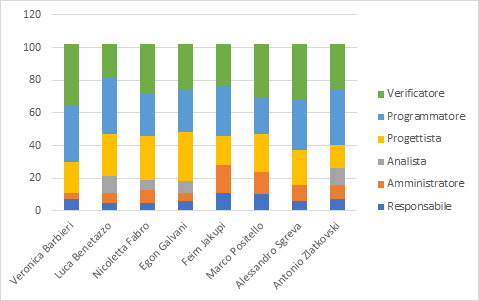
\includegraphics[width=0.7\textwidth]{./res/img/totaleRendicontate_po.png}
				\caption{Suddivisione oraria con il totale delle ore rendicontate}
			\end{figure}

		\newpage
		\subsubsubsection{Prospetto economico}
			Totale delle ore e costo per ciascun ruolo delle ore rendicontate:

			\rowcolors{2}{lightRowColor}{darkRowColor}
			\begin{longtable}{
				>{\centering}p{0.25\textwidth}
				>{\centering}p{0.05\textwidth}
				>{\centering\arraybackslash}p{0.15\textwidth} }

				\coloredTableHead
				\textbf{\color{white}Ruolo} &
				\textbf{\color{white}Ore} &
				\textbf{\color{white}Costo in \euro{}}
				\tabularnewline
				\endhead

				% Contenuto della tabella
				% Ruolo & Ore & Costo in \\
				Responsabile    & 57  & 1.710,00 \\
				Amministratore  & 73  & 1.460,00 \\
				Analista        & 33  & 825,00 \\
				Progettista     & 178 & 3.916,00 \\
				Programmatore   & 239 & 3.585,00 \\
				Verificatore    & 236 & 3.540,00 \\
				\textbf{Totale} & 816 & 15.036,00 \\

				\rowcolor{white}\caption {Prospetto dei costi totale delle ore rendicontate per ciascun ruolo} \\

			\end{longtable}

			\newpage
			% Grafico
			Rappresentazione grafica della distribuzione dei ruoli:
			\begin{figure}[h]
				\centering
				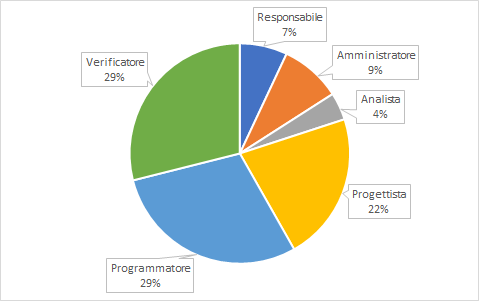
\includegraphics[width=0.7\textwidth]{./res/img/totaleRendicontate_pe.png}
				\caption{Suddivisione dei ruoli per il totale delle ore rendicontate}
			\end{figure}
